\documentclass[pdf, aspectratio=169]{beamer}
\usepackage[]{hyperref, graphicx, siunitx, lmodern, tikz, booktabs, physics,tensor}
\usepackage[mode=buildnew]{standalone}
\usepackage{pdfpc-commands}
\usepackage{intro-commands}

\usetheme{Astro}
\graphicspath{ {../Images/} }

\sisetup{per-mode=symbol}
\usetikzlibrary{calc, patterns, decorations.markings, decorations.pathmorphing, shapes}
\tikzstyle{proton}=[circle, minimum size = 7mm, ball color=red, black,transform shape]
\tikzstyle{neutron}=[circle, minimum size=7mm, ball color=gray, black, transform shape]
\tikzstyle{gammaray}=[ultra thick, -latex, decorate, decoration={snake, post length=3mm}]

%Preamble
\title{\ldots Please shine down on me!}
\author{Jed Rembold}
\date{October 22, 2018}

\begin{document}
\renewcommand{\theenumi}{\Alph{enumi}}

\begin{frame}{Announcements}
	\begin{itemize}
		\item Webwork due on Wednesday (just a single problem)
		\item Nothing due on Friday because\ldots
		\item Test 2 on Friday!!
			\begin{itemize}
				\item All review materials posted (with solutions)
				\item Equation page updated
				\item Email me if you want to reserve one of my few calculators for Friday
			\end{itemize}
		\item Lab Group B is meeting tonight for Exoplanets lab!
		\item Polling: \nolinkurl{rembold-class.ddns.net}
	\end{itemize}
\end{frame}

\begin{frame}{The Sky Tonight}
	\begin{itemize}
		\item Orionids Meteor shower!
			\begin{itemize}
				\item Technically peaked over the weekend
				\item Debris from Halley's comet
				\item Appear to originate in the constellation Orion
				\item Still visible (though at reduced rates) through the week
			\end{itemize}
	\end{itemize}
	\begin{center}
		\includegraphics[width=0.8\textwidth]{orionids_radiant.png}
	\end{center}
\end{frame}

\begin{frame}{Review Question!}
  What was one of the early barriers in determining the energy output (Luminosity) of the Sun?
  \begin{enumerate}
	\item \alert<2>{Determining its distance from Earth}
	\item Determining its angular size
	\item Determining what was powering it
	\item Determining the radius of the Earth
  \end{enumerate}
\end{frame}

\begin{frame}{Asking the Key Questions\ldots}
  \begin{itemize}
	\item Now that we understand the physical parameters of the Sun, we can attempt to answer some questions about it
	\item Most obviously:
  \end{itemize}
  \begin{center}
	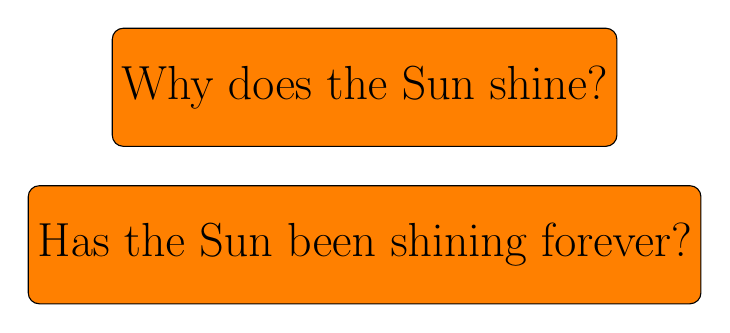
\begin{tikzpicture}
	  \node[rounded corners, minimum width=5cm, minimum height=1.5cm, fill=orange, draw=black, text=black, font=\LARGE] at (0,0) {Why does the Sun shine?};
	  \node[rounded corners, minimum width=5cm, minimum height=1.5cm, fill=orange, draw=black, text=black, font=\LARGE] at (0,-2) {Has the Sun been shining forever?};
	\end{tikzpicture}
  \end{center}
\end{frame}

\begin{frame}{Why so shiny?}
  \begin{itemize}
	\item Shining means the Sun is giving off energy
	\item Where it gets this energy was a major question of the early 1900s
	  \begin{itemize}
		\item Originally thought to be some sort of chemical burning
		  \begin{itemize}
			\item First estimates of the luminosity demanded WAY too much energy
			\item Would only have enough fuel for 16000 years
		  \end{itemize}
		\item Gravitational Contraction?
		  \begin{itemize}
			\item Could burn for 25 million years\ldots
			\item But Earth's fossil record indicates Earth is older than that?
		  \end{itemize}
	  \end{itemize}
  \end{itemize}
  \begin{center}
	\includegraphics[width=.3\textwidth]{ch11_shining_sun.png}
  \end{center}
\end{frame}

\begin{frame}{Stability}
  \begin{itemize}
	\item Regardless of energy source, why doesn't the Sun use up all it's fuel at once?
	\item If you light a match, it flares up and then burns out. No steady glow.
	\item<2-> Defying Gravity:
	  \begin{itemize}
		\item Gravity pulling everything inward
		\item Sun has not collapsed into a tiny ball over all these years
		\item Therefore, something must be working against gravity!
		  \begin{itemize}
			\item<3> \alert{Gas Pressure}
		  \end{itemize}
	  \end{itemize}
  \end{itemize}
\end{frame}

\begin{frame}{Under Pressure \scriptsize (dum dum dum bada dumdum)}
  \begin{itemize}
	\item We know molecules speed up when they get hot
	\item Pressure is a measure of how hard those molecules hit the edges of their container
	\item Hotter = Faster = More Energy = Harder Hitting
	\item So pressure and temperature are linked! (Among other things. Ideal Gas Law)
	\item As the Sun contracts, the warming molecules will push back with more force
	\item At some point, a balance is reached!
  \end{itemize}
  \begin{center}
	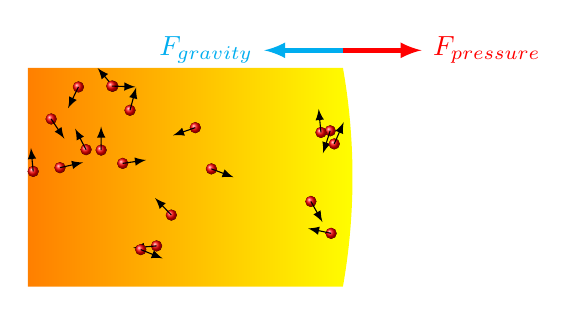
\begin{tikzpicture}[scale=1]
	  \shade[left color = orange, right color=yellow] (0,0) --++(4,0) arc (-10:10:8cm) --++(-4,0) -- cycle;
	  %\draw[ultra thick, orange] (4,0) arc (0:10:8cm);
	  %\draw[ultra thick, orange] (4,0) arc (0:-10:8cm);
	  \foreach \p in {1,2,...,20}{
		\fill[ball color=red] (rnd*4,rnd*2.6+.1) coordinate (p) circle (2pt);
		\draw[-latex, black] (p) --+(rnd*360:3mm);
	  }
	  \draw[ultra thick, cyan, -latex] (4,3) --+(-1,0) node[left] {$F_{gravity}$};
	  \draw[ultra thick, red, -latex] (4,3) --+(1,0) node[right] {$F_{pressure}$};
	\end{tikzpicture}
  \end{center}
\end{frame}

\begin{frame}{Gotta stay Balanced}
  \begin{columns}
	\column{.5\textwidth}
	  \begin{itemize}
		\item Everywhere in the star needs to be balanced
		\item The weight the pressure needs to support increases as we go deeper
		\item Pressure must therefore increase
		\item And thus temperature and density must also increase
	  \end{itemize}
	\column{.5\textwidth}
	\begin{center}
	  \begin{tikzpicture}[scale=.9, transform shape]
		\clip[rounded corners] (.1,.1) rectangle (4.5,7);
		\node[inner sep=0pt, outer sep=0pt, anchor=south west] at (0,0) {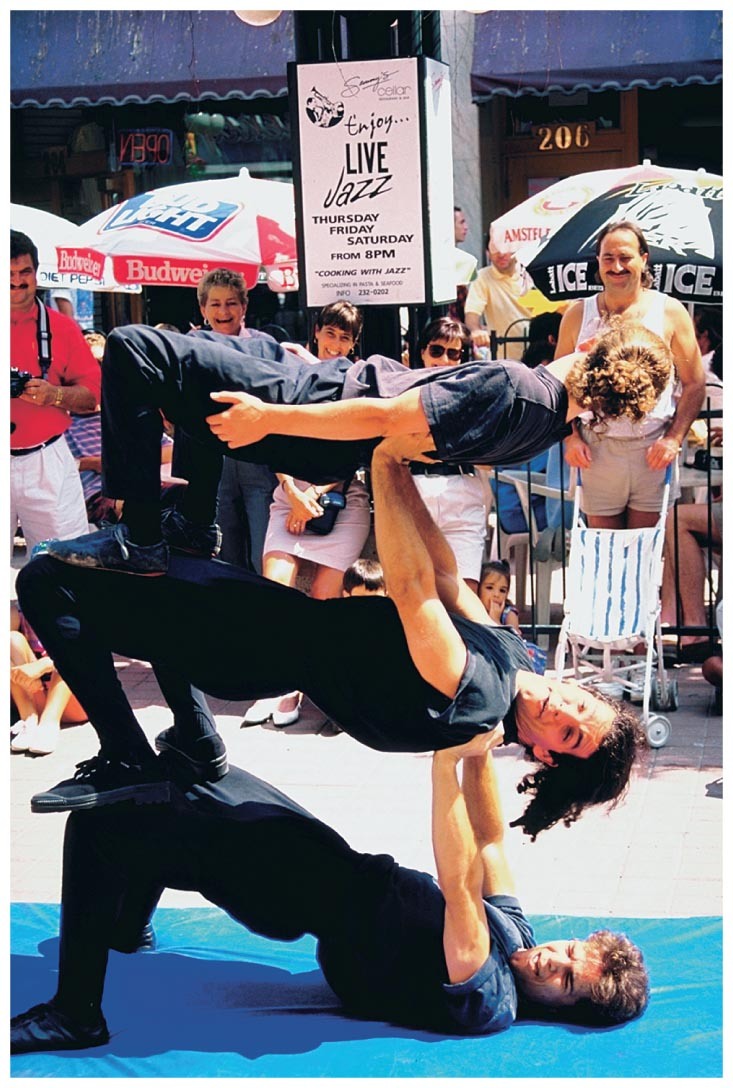
\includegraphics[width=.7\textwidth]{ch11_human_stack.jpg}};
	  \end{tikzpicture}
	\end{center}
  \end{columns}
\end{frame}

\begin{frame}{Even more balancing}
  \begin{itemize}
	\item Without an energy source, the Sun would slowly cool
	  \begin{itemize}
		\item Radiating energy out into the universe
	  \end{itemize}
	\item With too strong an energy source, the Sun would puff up and explode!
	  \begin{itemize}
		\item It couldn't emit the energy fast enough!
	  \end{itemize}
	\item Imagine a sealed hot air balloon
	  \begin{itemize}
		\item Heat the air too little and you'll cool and sink
		\item Heat the air too much and your balloon could pop
	  \end{itemize}
	\item The Sun is also therefore in \emph{energy balance}
	  \begin{itemize}
		\item Energy In = Energy Out
	  \end{itemize}
  \end{itemize}
\end{frame}

\begin{frame}{Providing Structure}
  \begin{columns}
	\column{.5\textwidth}
	\begin{itemize}
	  \item The Core
		\begin{itemize}
		  \item 15 million K
		  \item Where energy is created
		\end{itemize}
	  \item Radiation Zone
		\begin{itemize}
		  \item Energy moves slowly by photon emission (EM waves)
		  \item Think radiator heating
		\end{itemize}
	  \item Convection Zone
		\begin{itemize}
		  \item Hot gases rise, cold gases sink
		  \item Think boiling water
		\end{itemize}
	\end{itemize}
	\column{.5\textwidth}
	\begin{center}
	  \begin{tikzpicture}[scale=1.3, transform shape]
		\clip[rounded corners] (0,0) rectangle +(5,5);
		\node[inner sep=0pt, outer sep=0pt, anchor=south west] {\includegraphics[width=5cm]{ch11_sun_structure.jpg}};
	  \end{tikzpicture}
	\end{center}
  \end{columns}
\end{frame}

\begin{frame}{Providing More Structure}
  \begin{columns}
	\column{.5\textwidth}
	\begin{itemize}
	  \item Photosphere
		\begin{itemize}
		  \item Around 6000 K
		  \item Visible ``surface'' of Sun
		\end{itemize}
	  \item Chromosphere
		\begin{itemize}
		  \item Thin layer just above photosphere
		  \item Radiates mostly ultraviolet
		\end{itemize}
	  \item Corona
		\begin{itemize}
		  \item Extremely hot: around 1 million K
		  \item Density very low
		\end{itemize}
	\end{itemize}
	\column{.5\textwidth}
	\begin{center}
	  \begin{tikzpicture}[scale=1.3, transform shape]
		\clip[rounded corners] (0,0) rectangle +(5,5);
		\node[inner sep=0pt, outer sep=0pt, anchor=south west] {\includegraphics[width=5cm]{ch11_sun_structure.jpg}};
	  \end{tikzpicture}
	\end{center}
  \end{columns}
\end{frame}

\begin{frame}{We need more \emph{power} Captain!}
  \begin{itemize}
	\item The quest to determine from whence the Sun gains its power:
	  \begin{itemize}
		\item 1890's: Radioactivity discovered
		  \begin{itemize}
			\item Elements can transform from one to another and release energy in the process
		  \end{itemize}
		\item 1905: Einstein's Special Relativity
		  \begin{itemize}
			\item Mass and energy are equivalent
			\item $E = mc^2$
		  \end{itemize}
		\item 1930's: Discovery of the Neutron
		  \begin{itemize}
			\item Understanding H and He nuclei
		  \end{itemize}
		\item 1939: Hans Bethe worked out a detailed mechanism for the Sun's power source
	  \end{itemize}
  \end{itemize}
\end{frame}

\begin{frame}{Going Nuclear}
  \begin{itemize}
	\item To understand our Sun's energy production, we need to focus on the tiny:
	  \begin{itemize}
		\item Elements on the Periodic Table are comprised of Protons, Neutrons, and Electrons
		\item There are 4 main forces we know that describe the universe:
		  \begin{itemize}
			\item The Strong Nuclear Force binds atoms
			\item The Weak Nuclear Force governs radioactive decay
			\item The Electromagnetic Force covers charges and magnets
			\item The Gravitational Force covers mass attraction
		  \end{itemize}
		\item At the atomic level, the gravitational force is irrelevant
		\item The strong nuclear force is the strongest of the fundamental forces, but incredibly small in range (Think femtometers = $10^{-15}$ meters)
	  \end{itemize}
  \end{itemize}
\end{frame}

\begin{frame}{Proton Packing}
  \begin{itemize}
	\item Protons are positively charged
	\item Putting positively charged things next to each other makes them want to repel (Electromagnetic force)
	\item So to make an atom, you need to manage to squeeze them close enough together to let the stronger nuclear force ``grab'' them, despite the electromagnetic force pushing them away
	\item If your atom gets too large, then your strong nuclear force will weaken, making it easier for protons to escape
	\item Since $E=mc^2$, you can actually measure this ``energy of binding'' by comparing the masses of the individual atoms to the mass of the combined element!
  \end{itemize}
\end{frame}

\begin{frame}{Binding Energy}
  The amount of energy needed to hold elements together varies!
  \begin{center}
	\begin{tikzpicture}
	  \begin{axis}[
		  width=\textwidth,
		  height=6cm,
		  xlabel = Mass Number (Neutrons + Protons),
		  ylabel = Binding Energy (MeV),
		]
		\addplot[scatter] table {../Data/BindingEnergy.csv};
		\node[pin=-90:Iron] at (axis cs: 56,8.5) {};
		\node[pin=45:Hydrogen] at (axis cs: 1,1) {};
		\node[pin=250:Uranium] at (axis cs: 238,7.3) {};

		\fill<2>[cyan, opacity=.5] (axis cs: 0,0.7) rectangle (axis cs: 56,9);
		\node<2>[white] at (axis cs: 28,4) {Fusion};
		\fill<3>[orange, opacity=0.5] (axis cs: 56,0.7) rectangle (axis cs: 250,9);
		\node<3>[white] at (axis cs: 147,4) {Fission};
	  \end{axis}
	\end{tikzpicture}
  \end{center}
\end{frame}

\begin{frame}{Fusion Power!}
  \begin{itemize}
	\item The interior of the Sun is very dense, very hot, and very Hydrogen
	\item Packs lots of protons close together and moving real fast
	\item When protons get close enough:
	  \begin{itemize}
		\item Bang! Fusion happens!
		\item Energy is given off!
		\item The cycle continues\ldots
	  \end{itemize}
  \end{itemize}
\end{frame}

%\begin{frame}{Powering Your Sun: A 3 Step Process}
  %\begin{center}
	%\begin{tikzpicture}
	  %\onslide<1->{
		%\coordinate (col1) at (1,0);
		%\draw[ultra thick, cyan, -latex] (0,2) node[proton] {p} -- (col1);
		%\draw[ultra thick, cyan, -latex] (0,-2) node[proton] {p} -- (col1);
		%\draw[ultra thick, orange, -latex] (col1) --+(60:1.5) node[right] {$e^+$};
		%\node[proton] (p1) at ($(col1)+(2,0)$) {p};
		%\node[neutron] (n1) at ($(p1)+(4mm,0)$) {n};
		%\draw[ultra thick, orange, -latex] (col1) --(p1);
		%\draw[ultra thick, orange, -latex] (col1) --+(-60:1.5) node[right] {$\nu$};
	  %}
	  %\onslide<2->{
		%\draw[ultra thick, cyan, latex-] (n1) --+(-100:2) node[proton] {p};
		%\node[proton](p2) at ($(n1)+(2,0)$) {p};
		%\node[proton] at ($(p2)-(0,4mm)$) {p};
		%\node[neutron](n2) at ($(p2)+(-30:4mm)$) {n};
		%\draw[orange, ultra thick, -latex] (n1) -- (p2);
		%\draw[orange, gammaray] (n1) --+(60:2) node[right] {$\gamma$};
		%\fill[Background, opacity=0.6] (-1,-3) rectangle (2.6,3);
	  %}
	  %\onslide<3->{
		%\node[proton](p3) at ($(p2)+(0,-2)$) {p};
		%\node[proton] at ($(p3)-(0,4mm)$) {p};
		%\node[neutron](n3) at ($(p3)+(-30:4mm)$) {n};
		%\draw[ultra thick, cyan, -latex] (p3) -- (n2);
		%\draw[ultra thick, orange, -latex] (n2) --+(60:2) node[anchor=south west,proton] {p};
		%\draw[ultra thick, orange, -latex] (n2) --+(-60:2) node[anchor=north west,proton] {p};
		%\draw[ultra thick, orange, -latex] (n2) --+(2,0) node[anchor=west, proton] (p4) {p};
		%\node[neutron] at ($(p4)+(60:4mm)$) {n};
		%\node[proton] at ($(p4)+(0:6mm)$) {p};
		%\node[neutron] at ($(p4)+(-60:4mm)$) {n};
		%\fill[Background, opacity=0.6] (-1,-3) rectangle (5,3);
	  %}
	%\end{tikzpicture}
	%\onslide<3->{\[4\left( \nuclide[1][1]{H} \right) \rightarrow \nuclide[4][2]{He} + 2e^+ + 2\nu + \gamma\]}
  %\end{center}
%\end{frame}

%\begin{frame}{End Products}
  %\begin{columns}
	%\column{.5\textwidth}
	%\begin{itemize}
	  %\item 1 He nucleus (2 protons, 2 neutrons)
	  %\item 2 $e^+$ (positrons or anti-electrons)
		%\begin{itemize}
		  %\item Will ``annihilate'' with electrons, releasing energy via gamma rays
		%\end{itemize}
	  %\item 2 $\nu$ (neutrinos)
		%\begin{itemize}
		  %\item No charge
		  %\item Very, very low mass
		  %\item Very non-interactive (only through weak force and gravity)
		%\end{itemize}
	%\end{itemize}
	%\column{.5\textwidth}
	%\begin{center}
	  %\begin{tikzpicture}
		%\node[neutron] (n1) at (0,0) {n};
		%\node[neutron] (n2) at ($(n1)+(0,-7mm)$) {n};
		%\node[proton] (p1) at ($(n1)+(225:5mm)$) {p};
		%\node[proton] at ($(p1)+(7mm,0)$) {p};
		%\foreach \a in {25,70,115,160}{
		  %\draw[ultra thick, cyan, latex-] (n1) --+(\a:2) node[proton] {p};
		%}
		%\foreach \a in {190,280}{
		  %\draw[orange, gammaray] (n2) --+(\a:2) node[below] {$\gamma$};
		  %\draw[orange, ultra thick, -latex] (n2) --+({\a+30}:2) node[below] {$e^+$};
		  %\draw[orange, ultra thick, -latex] (n2) --+({\a+60}:2) node[below] {$\nu$};
		%}
	  %\end{tikzpicture}
	%\end{center}
  %\end{columns}
%\end{frame}

%\begin{frame}{Energy Scales}
  %\begin{itemize}
	%\item The mass of 1 He nucleus is \alert{slightly} less than the mass of 4 H nuclei
	  %\begin{itemize}
		%\item Mass of He is 3.97 proton masses
		%\item About 3\% of a proton mass has gone somewhere!
		%\item The positrons do not account for it!
	  %\end{itemize}
	%\item This mass has been converted to energy
	  %\begin{itemize}
		%\item $E=mc^2$
		%\item About \SI{4.2e-12}{\joule}
		%\item Energy carried away by the gamma rays and neutrinos
	  %\end{itemize}
  %\end{itemize}
  %\begin{center}
	%\begin{tikzpicture}[scale=.5]
	  %\coordinate (tray1) at (-3,1);
	  %\coordinate (tray2) at (3,2);
	  %\fill[gray] (tray1) --++(2,0) coordinate (c1e) --++(-1,-1) --++(-2,0) --++(-1,1) coordinate (c1w) --cycle;
	  %\draw (c1e) -- ($(tray1)+(0,3)$) coordinate (peak1) -- (c1w);
	  
	  %\fill[gray] (tray2) --++(2,0) coordinate (c2e) --++(-1,-1) --++(-2,0) --++(-1,1) coordinate (c2w) --cycle;
	  %\draw (c2e) -- ($(tray2)+(0,3)$) coordinate (peak2) -- (c2w);

	  %\draw[line width=3pt, line cap=round] (peak1) -- coordinate[pos=0.5] (mid) (peak2);
	  %\draw[line width=3pt] (mid)--+(0,-5) coordinate (base);
	  %\draw[line width=5pt, line cap=round] (base) --+(1,0) (base) --+(-1,0);

	  %\foreach \x in {1,2,3,4}{
		%\node[proton] at ($(tray1)-(20mm,0)+(\x*8mm,0)$) {p};
	  %}

	  %\node[proton] (p1) at (tray2) {p};
	  %\node[proton] at ($(p1)+(0,7mm)$) {p};
	  %\node[neutron] at ($(p1)+(-3.5mm,3.5mm)$) {n};
	  %\node[neutron] at ($(p1)+(3.5mm,3.5mm)$) {n};
	  %\node[align=center, anchor=south, font=\tiny] at ($(tray2)+(-1,0)$) {$e^+$\\$e^+$};
	  %\node[align=center, anchor=south, font=\tiny] at ($(tray2)+(1,0)$) {$\nu$\\$\nu$};
	%\end{tikzpicture}
  %\end{center}
%\end{frame}

%\begin{frame}{Taking things slow\ldots}
  %\begin{itemize}
	%\item The full 3 step reaction is actually quite slow!
	%\item First Step:
	  %\begin{itemize}
		%\item The tricky one
		%\item Need both to get \alert{really} close AND need the proton to decay into a neutron
		%\item Takes over a billion years!
	  %\end{itemize}
	%\item Second Step:
	  %\begin{itemize}
		%\item Quite fast
		%\item About 1 second
	  %\end{itemize}
	%\item Third Step:
	  %\begin{itemize}
		%\item Slow again, but 1000$\times$ faster than Step 1
		%\item About a million years
	  %\end{itemize}
	%\item The sheer number of protons is what keeps such a high energy output!
  %\end{itemize}
%\end{frame}





\end{document}

